\subsection{Etat de l'art}

\subsection{Formalisme}

\subsection{Initialisation}

\subsection{Implémentation}
    L'implémentation d'un \gls{Plugin} \gls{Gazebo} permet ainsi de simuler le comportement de l'ombilical dans l'environnement de simulation. Ce plugin est basé sur la programmation orientée objet et permet d'instancier un objet de type \textsc{Tether} et des objets \textsc{TetherElement}. La \textsc{Tether} utilise une structure de liste doublement chaînée\footnote{structure de données liée qui consiste en un ensemble n\oe uds liés les uns aux autres par des références au n\oe ud précédente et au n\oe ud suivant.} de \textsc{TetherElement}, et n'a en mémoire que le premier et le dernier n\oe ud de la chaîne, nommés \textsc{head} et \textsc{tail}. Il est ensuite possible de parcourir les différents \textsc{TetherElement} en utilisant les références gardées en mémoires par les \textsc{TetherElement} eux-mêmes. Un diagramme de classe est présenté en \textsc{Figure}~\ref{fig:uml_class}.

    \begin{figure}[!htb]
        \centering
        \resizebox{0.90\textwidth}{!}{
            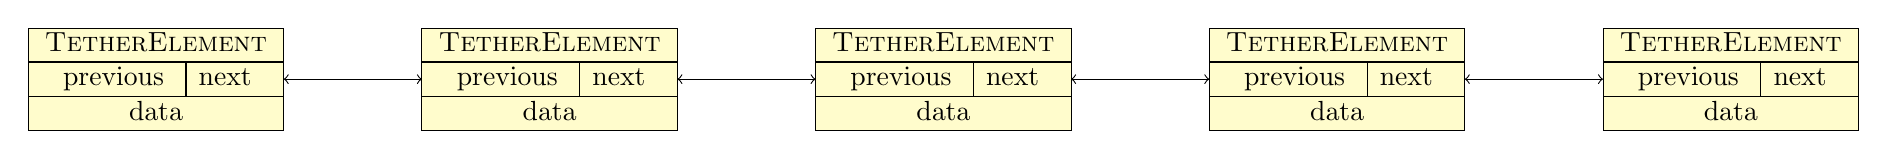
\begin{tikzpicture}
                \tikzset{TE/.style={draw, inner sep=0, outer sep=0, fill=yellow!20}}

                \foreach \i in {1,...,5} {
                    \node[TE] (TE\i) at (5*\i,0) {\begin{tabular}{c} \textsc{TetherElement} \\ \hline \hfill previous \hfill \vline \hfill next \hfill \\ \hline data \end{tabular}};
                }
                
                \foreach \i in {1,...,4} {
                    \pgfmathtruncatemacro{\next}{\i +1}
                    \draw[<->] (TE\i) -- (TE\next);
                }

            \end{tikzpicture}
        }
        \caption{Doubly Linked List}
        \label{fig:doubly_linked_list}
    \end{figure}

    \begin{figure}[!htb]
        \centering
        \resizebox{0.50\textwidth}{!}{
            \begin{tikzpicture}
                \begin{class}[text width=6cm]{Tether}{0,0}
                    \attribute{+ element\_mass : double}
                    \attribute{+ element\_volume : double}
                    \attribute{+ element\_length : double}
                    \attribute{+ position\_first : numpy.ndarray}
                    \attribute{+ position\_last : numpy.ndarray}
                    \attribute{+ elements : list of \textit{TetherElement}}
                \end{class}
            
                \begin{class}[text width=6cm]{TetherElement}{8.5,0}
                    \attribute{+ mass : double}
                    \attribute{+ volume : double}
                    \attribute{+ length : double}
                    \attribute{+ position : numpy.ndarray}
                    \attribute{+ velocity : numpy.ndarray}
                    \attribute{+ acceleration : numpy.ndarray}
                    \attribute{+ previous : TetherElement}
                    \attribute{+ next : TetherElement}
                    \attribute{+ K\_p : double}
                    \attribute{+ K\_d : double}
                    \attribute{+ K\_i : double}
                    \operation{+ F\_p(self) : numpy.ndarray}
                    \operation{+ F\_b(self) : numpy.ndarray}
                    \operation{+ F\_f(self) : numpy.ndarray}
                    \operation{+ Ft\_prev(self) : numpy.ndarray}
                    \operation{+ Ft\_next(self) : numpy.ndarray}
                \end{class}
            
                \aggregation{Tether}{}{~~~n}{TetherElement}
            \end{tikzpicture}
        }
        \caption{UML diagram of the \textit{Tether} and \textit{TetherElement} classes}
        \label{fig:uml_class}
    \end{figure}

\subsection{Suivi d'angles normalisés}
    Un problème avec la représentation numérique de l'orientation des solides est qu'elle est souvent normalisée, et les valeurs sont ainsi ramenées dans l'intervalle $[-\pi; \pi]$. On ne peut donc pas avoir l'orientation absolue, c'est à dire l'orientation d'un solide en prenant en compte les eventuels tours qu'il aurait pu faire sur lui-même.

    Pour résoudre ce problème, l'\textsc{Algorithme}~\ref{algo:suivi_angle} de suivi d'angles normalisés a été implémenté. Il prends en paramètres l'angle normalisé ainsi que l'angle précédemment calculé, et il retourne la valeur de l'angle absolu. L'idée de fournir l'angle précédent est de pouvoir retourner le nouvel angle qui se trouve dans le même quadrant et aussi de pouvoir suivre les sauts d'angles. Ainsi on peut suivre l'orientation absolue de solides en rotation dans l'espace, en ne fournissant que des orientations relatives ramenées dans l'intervalle $[-\pi; \pi]$, et en gardant en mémoire la précédente orientation calculée.
    
    \begin{algorithm}[!htb]
        \SetKwInOut{Input}{Entrées}
        \SetKwInOut{Output}{Sorties}
        \Entree{$angle\_normalise$, $angle\_absolu$}
        \Sortie{$angle\_absolu$}
        \Deb{
            $offset \leftarrow (angle\_absolu - angle\_normalise + \pi ) \pmod{2\pi}$ \\
            $angle\_absolu \leftarrow angle\_normalise + 2\pi \cdot offset$ \\
        }
        \Retour{$angle\_absolu$}

        \caption{Suivi d'angle} 
        \label{algo:suivi_angle}
    \end{algorithm}

    La \textsc{Figure}~\ref{fig:suivi_angle} présente les résultats de l'\textsc{Algorithme}~\ref{algo:suivi_angle} avec une angle variant dans l'intervalle $[-3\pi; 3\pi]$. On voit sur la première sous-figure l'angle réel et l'angle ramené dans l'intervalle $[-\pi; \pi]$ avec la présence de saut d'angles. Avec cette méthode, on est capable de suivre l'évolution de l'angle et de supprimer cess sauts afin de retrouver l'angle absolu visible dans la deuxième sous-figure et calculé uniquement à partir de la connaissance de l'angle normalisé.

    \begin{figure}[!htb]
        \centering
        \includegraphics[width=0.5\textwidth]{suivi_angle.png}
        \caption{Suivi d'angle}
        \label{fig:suivi_angle}
    \end{figure}


\subsection{Resultats}